\documentclass[12pt]{report}
\usepackage[utf8]{inputenc}
\usepackage{amsmath}
\usepackage{amsfonts}
\usepackage{amssymb}
\author{Edward Seabrook} 
\title{Third Year Project Final Report}

\usepackage{nomencl}
\makenomenclature

% Makes Chapter heading look like Section heading
\usepackage{titlesec}
\titleformat{\chapter}% reformat chapter headings
    [hang]% like section, with number on same line
    {\Large\bfseries}% formatting applied to whole
    {\thechapter}% Chapter number
    {0.5em}% space between # and title
    {}% formatting applied just to title

% Save a bit of space by giving all headings less room
\titlespacing*{\chapter}{0pt}{0pt}{0pt}
\titlespacing*{\section}{0pt}{0pt}{5pt}
\titlespacing*{\subsection}{0pt}{0pt}{5pt}
\titlespacing*{\subsubsection}{0pt}{0pt}{5pt}
\titlespacing*{\paragraph}{0pt}{0pt}{5pt}

% Set margins to required
\usepackage[top=2.4cm, bottom=2.4cm, left=3.5cm, right=2.4cm]{geometry} 

% Sort out margins for todonotes
\setlength{\marginparwidth}{3cm}
\reversemarginpar

% Set paragraph spacing to required
\setlength\parindent{0pt}
\usepackage[parfill]{parskip}

\usepackage{hyperref}
\usepackage{todonotes}
\usepackage{listings}
\usepackage{appendix}
\usepackage{pdflscape}
\usepackage{cite}

\hypersetup{colorlinks=false, pdfborder={0 0 0}, }

% Not totally sure
\usepackage{fancyhdr} 
\pagestyle{fancy} 
\renewcommand{\headrulewidth}{0pt} 
\lhead{}\chead{}\rhead{}
\lfoot{}\cfoot{\thepage}\rfoot{}

% Number and show in ToC to a deeper level
\setcounter{secnumdepth}{3}
\setcounter{tocdepth}{3}

\def\nomlabel#1{\textbf{#1}\hfil}

\begin{document}

% Include title page

\begin{titlepage}

\begin{center}


% Upper part of the page
%\includegraphics[width=0.15\textwidth]{./logo}\\[1cm]    

\LARGE Electronics and Computer Science\\
Faculty of Physical and Applied Sciences\\
University of Southampton
\\[1.5cm]

\href{mailto:ejfs1g10@ecs.soton.ac.uk}{Edward JF Seabrook}\\[0.5cm]

\today \\[1cm]
{\bfseries A Tool to Simplify Network Administration in the Modern Home}\\[1.5cm]

\vfill

% Author and supervisor
\large
Project Supervisor: 
Dr.~T \textsc{Chown}\\

\large
Secondary Examiner:
Dr.~KP \textsc{Zauner} 

\vfill

A Project Progress Report Submitted for the Award of Computer Science

\end{center}

\end{titlepage}


\begin{abstract}
As home networks become more and more complex, it is inevitable that they will
require splitting into multiple subnets. As the average home user is unable to
configure a router, a minimal configuration solution is required. In this
project I produced an implementation of zero configuration OSPF based on drafts
published by the IETF\@\nomenclature{IETF}{Internet Engineering Task Force}. 
\end{abstract}

\tableofcontents
\clearpage

\chapter*{Acknowledgements}
\todo{Write as prose}
I would like to thank the following people for all their help, support and
influence during this project:
\begin{itemize}
\item Tim Chown - Offered support as project supervisor
\item David Lamparter - Responded to my queries about how Quagga works
\item Jari Arkko - Wrote the drafts that I was implementing
\item Markus Stenberg \& Benjamin Paterson - Provided implementations against which 
      to interop test
\item Friends \& Family for proof reading this document.
\end{itemize}

\chapter{Introduction}
\todo{A clear statement of the problem and goals of the project.}
The title of my project is ``Implementing Zero Configuration OSPFv3''. During
the project, I have modified an open source implementation of the OSPFv3
routing protocol to comply with two recently published, and very topical,
internet drafts. The changes allow routed networks to be set up without the
need for manual configuration.

\section{The Problem}
As computing becomes more and more ubiquitous the complexity of an average home
network will increase. Not only will the number of devices rise, but with the
advent of sensor networks and home automation, the quantity of types and
topologies present will grow. To ensure these more complex networks run
smoothly, they should be separated into multiple subnets. Routing is required
to allow communication between these subnets. 

Unfortunately, the vast majority of home networks do not have a professional
System Administrator, or other sufficiently computer literate person, around to
configure and maintain them. This means ideally a network should not require any
manual configuration to work.

A less relevant, but equally, if not more serious issue that is addressed in
this project is IPv4 \nomenclature{IPv4}{Internet Protocol Version 4} address
space exhaustion. 

\section{The Goals}
This project set out to meet many goals, over the course of the project, as my
understanding of the problem improved, the goals have transformed slightly.

\subsection{Project Goals}
The goals for the project are:

\begin{itemize}
\item Allow multiple subnets in the home; allow hosts to communicate from one
  subnet to another.
\item Distribute IPv6 subnet prefixes across a home network in an efficient
	manner. 
\item Require no configuration: The user should not need to enter any settings,
  they should simply plug in the router, and it should work.
\item Produce something of value for the community. The code I produce should
  adhere to style and quality guidelines to ensure it is useful.
\item Verify past implementations of the drafts.
\item Discover any ambiguities in the drafts.
\end{itemize}

\subsection{Personal Goals}
I also had a set of personal goals that I aimed to achieve over the course of
the project:
\begin{itemize}
	\item Develop a good understanding of the OSPF routing protocol.
	\item Improve my understanding of the process of the creation of internet
		standards.
	\item Obtain the ability to implement network protocols.
	\item Increase my programming ability (Mainly C or C++).
	\item Learn about new tools and techniques.
\end{itemize}

\chapter{Background}
\todo{Is this section a big waffle?}
To enable me to explain my project in detail, I first need to explain the
concepts that it is based on.

\section{Home Networks}
Modern home and small/home office (SOHO) \nomenclature{SOHO}{Small Office Home
Office} networks tend to follow the same pattern. A single ISP provides a
connection to the internet using the phone line or television cable.  The ISP
will typically provide a single IPv4 address (/32), usually this is an unstable
(dynamic) allocation - a static IP is often offered as a premium service. 

To allow multiple hosts on the network, Network Address Translation (NAT)
\nomenclature{NAT}{Network Address Translation} is usually employed. With NAT,
the router rewrites the address of the packets from the global IP address to a
local IP address. The address range 192.168.1.0/24 is often used for these
local IP addresses. Ports number are often used to multiplex between the
different hosts and applications on the network. To allow programs like Skype
to function, Universal Plug and Play (UPnP) \nomenclature{UPnP}{Universal Plug
and Play}, a technology that allow automatic port mapping on a network, is
frequently deployed. Local IP addresses are assigned to the hosts by the router
using the Dynamic Host Configuration Protocol (DHCP)\nomenclature{DHCP}{Dynamic
Host Configuration Protocol}. 

A single item of Customer Premises Equipment (CPE) \nomenclature{CPE}{Customer
Premises Equipment} is usually supplied to the customer. These devices are
referred to by many names\footnote{Names include Super Hub, HomeHub and
WirelessBox}, commonly as a ``Router''.  This device provides the modem for
connecting to the internet, an Ethernet switch with around four ports, and a
wireless access point (802.11) that tends to be bridged to the wired network to
provide just one subnet. A diagram of a typical home network can be seen in
Appendix~\ref{typical_homenet_present}.

\section{Campus and Enterprise Networks}
Larger networks like the ones found on University Campuses and larger
businesses tend to employ many of the more advanced features of networking.
They are often split into multiple subnets separating the physical locations,
work groups and expected use of the hosts. One potential corporate network
topology can be seen in Appendix~\ref{typical_corporate_net}.

\todo{Is there any evidence to support this?}
In the early days of the internet, many organisations were able to obtain large
chunks of IPv4 address space - MIT famously has the control of a /8 address
range. The University of Southampton was able to obtain a /16 (152.78.0.0)
giving them around 65000 addresses to play with. Having this many addresses
allows each machine on the network to be globally addressable - at first this
may seem to be insecure, but a good firewall is far more effective protection
than NAT\@. Even with this many addresses, the University still struggles. This
is due at part to address space wastage, the now deprecated ISS wireless
service still takes up a large proportion of the address space.

Although it is not yet common place, the networks run by ECS are dual stack,
the machines are allocated both IPv4 and IPv6 addresses. The 6th June 2012 was
the World IPv6 Launch, on this day many websites, including Facebook and
Google, began offering IPv6 connectivity to their users. This demonstrates than
IPv6 is mature enough to be deployed in large networks.

It should be noted however, to run a network the size of the University's,
based on todays technology, many specialist staff are required to configure the
network and ensure its day to day running. This is something that the vast
majority of households are not able to obtain.

\section{Future Networks}
In the future users will expect more from their home networks. We are likely to
see a dramatic increase in the number of devices in the average home, ranging
from more laptops, smart phones and tablets, to more sensors and home automation
devices. A hypothetical home network of the future is depicted in
Appendix~\ref{typical_homenet_future}.

A home network with this quantity and heterogeneity of traffic is likely to
experience slow downs and other issues. These problems arise for two reasons:
Firstly networks such as sensor networks run very slowly, where as Gigabit
Ethernet networks run very quickly - this difference in speed can result in
both networks running even slower. The other issue is the vast amounts of
multicast and broadcast traffic that will build up on networks with many
devices performing functions such as service discovery. It would be beneficial
to split the network up into multiple subnets to ensure the best performance
from each network. 

Guest networks are already an option provided by some high end wireless access
points. By using Virtual Access Points (VAPs) \nomenclature{VAP}{Virtual Access
Point} guest clients can connect to the internet, but are restricted from
having full access to the local network. To facilitate this, hard coded local
IPv4 addresses are usually used, with the advent of IPv6 and globally valid
addresses, a mechanism to assign IP addresses and route traffic is required. 

The Internet Engineering Task Force's (IETF) Homenet working group
\cite{homenet} are working on the architecture of the home network of the
future. Their work mainly focuses on addressing, routing, topology and security
in home networks. 

\section{IPv6}
To communicate with a computer, we need a way of uniquely identifying it. At
present, IPv4 is the dominant technology for addressing computers on the
internet. Unfortunately when IPv4 was designed, it was not foreseeable that we
would need more than 4 billion addresses, so a neat 32 bit identifier was used.
In 2011 however, The Internet Assigned Numbers Authority (IANA)
\nomenclature{IANA}{Internet Assigned Numbers Authority} ran out of IPv4
addresses. 

One solution to the IPv4 address space exhaustion problem is migration to
IPv6; a protocol that is fundamentally similar to IPV4, but instead uses 128
bit addresses. This gives us far more addresses to work with - in fact a total
of $3.4028237\times10^{38}$ unique addresses. With estimates for the total
number of grains of sand on Earth being around $7.5\times10^{18}$, the number
of stars visible from Earth falling at about $7.0\times10^{22}$, and the
estimated human population of Earth being a mere $7.0\times10^{9}$,
this address space should be sufficient for at least the foreseeable future. 

IPv6 address ranges are often given in Classless Inter-Domain Routing (CIDR)
\nomenclature{CIDR}{Classless Inter-Domain Routing} notation. In this notation
an IPv6 address is written, followed by a slash and then and number between 0
and 128. This number represents the number of bits in the IPv6 address that
identify the network, and the rest of the bits identify the host.

IPv6 prefixes tend to be /64, as this is required by Stateless Address
Autoconfiguration (SLAAC)\nomenclature{SLAAC}{Stateless Address
Autoconfiguration}. A /48 prefix may be allocated by an ISP to allow the user
to assign multiple subnets on their network.

\section{Routing}
For packets of data to find their way between subnets, they require routing.
The routing we are concerned with is Layer 3 routing. When an IP packet is
sent, its address is compared with those stored in the kernel's routing table,
and then transmitted using the appropriate interface. Networks contain many
computers, known as routers,  whose sole purpose is to forward network traffic.

A number of different protocols exist to build up these routing tables:

\subsection{Interior gateway protocols}
Interior Gateway Protocols (IGPs) \nomenclature{IGP}{Interior Gateway
Protocols} are concerned with building the routing tables for a single
autonomous system (AS) \nomenclature{AS}{Autonomous System}. ASs are generally
managed by ISPs or other very large organisations.  

\subsubsection{Distance Vector}
Distance vector routing works by having each router advertise to its neighbors
(directly connected routers) the shortest path it knows about to each subnet.
Although less complex that link-state routing protocols, they are often slower
to converge, and experience what is know as the ``count to infinity'' problem
whereby loops in the network topology can lead to weights increasing to
infinity when a router goes down. 

The most common Distance Vector protocol is Routing Information Protocol (RIP)
\nomenclature{RIP}{Routing Information Protocol}, a routing protocol famous for
defining 15 as infinity. The most recent revision is RIP Next Generation
(RIPng) which offers IPv6 support. IGRP and EIGRP are Cisco's own propriety
alternatives.

\subsubsection{Link-State}
Link state routing protocols work by allowing each router on the network to get
a full understanding of the network topology. From this representation of the
networks topology, the router then performs some calculations to work out the
best routes. The two most common Link-State routing protocols, Open Shortest
Path First (OSPF) \nomenclature{OSPF}{Open Shortest Path First} and
Intermediate System to Intermediate System (IS-IS)
\nomenclature{IS-IS}{Intermediate System - Intermediate System}, both use
Dijkstra's algorithm to calculate these shortest paths. 

OSPF and IS-IS are both very similar protocols, the main difference is that
IS-IS as a Layer 2 protocol is Layer 3 agnostic, whereas OSPF is dependent on
IPv4 or IPv6 depending on the version.

\subsection{Exterior Gateway Protocols}
Exterior Gateway Protocols (EGP) \nomenclature{EGP}{Exterior Gateway Protocol}
are used to establish peerings between ASs. EGPs typically run only on edge
routers and construct the route tables based on policy rather than the
technical distance of the destinations. In this project I was not concerned
with this kind of routing protocol.  The most widely used EGP today is Border
Gateway Protocol (BGP) \nomenclature{BGP}{Border Gateway Protocol}.

\chapter{Literature Review} 
The project was based on two closely related internet drafts, they were both
published very recently, and have the same authors. If these drafts are
approved by the IETF they will end up becoming Request for Comments
(RFC)\nomenclature{RFC}{Request for Comments}, the technical documents that
specify how the internet works. As RFCs these documents will be placed on the
standards track and will be labeled as ``Proposed Standards''. If they are
successful in meeting certain criteria, they may eventually become ``Internet
Standards''\cite{rfc6410}.

\section{OSPFv3 Autoconfiguration}
This draft\cite{draft-ietf-ospf-ospfv3-autoconfig-02} describes how OSPF for
IPv6 can be extended to run without requiring configuration. The draft begins
by enforcing some default values, and restricting a few features - such as
allowing only the backbone area to be used. It then specifies a mechanism for
generating Router IDs and ensuring that there are no conflicts across the
network. This is achieved by the introduction of a new Link State Advertisement
(LSA) \nomenclature{LSA}{Link State Advertisement} type. 

The most recent release of this document was on 15th April 2013. Although this
was towards the end of my project, the changes were only minor and I was able
to incorporate them into my implementation.

\section{OSPFv3 Prefix Assignment}
Building on the work of the Autoconfiguration draft, this
draft\cite{draft-arkko-homenet-prefix-assignment-03} solves the issue of
delegating IPv6 network prefixes from a larger pool of IPv6 addresses. As well
as offering a realistic solution to a problem, the draft also demonstrates the
extensibility of the Autoconfiguration draft. 

A method for breaking up a short prefix delegation into many network prefixes
is given, along with a strategy for avoiding conflicts across the network.
Typically an ISP will allocate a customer a /48 IPv6 prefix to cover their
whole home, each network in their home then requires a /64 IPv6 prefix.

An update to this document was published on 23rd October 2013, it expired on
26th April 2013, although it is likely a refresh will be released soon.

\section{Other Important Drafts}
There are several other documents that are relevant to this project. These are
both articles that are relevant as background knowledge and papers that have
been referenced from one another.

\subsection{Home Networking Architecture for IPv6} 
This paper\cite{draft-ietf-homenet-arch-07} puts forward a vision of future
home networking. An architecture for future home networks is proposed, along
with a discussion of emerging technologies. 

\subsection{OSPF Version 2}
I studied RFC2328\cite{RFC2328} in depth to understand the OSPF Protocol. The
memo is surprisingly easy to read, and offers a complete discussion of the data
structures and algorithms the OSPF protocol employs to build routing tables for
IPv4. 

Although the document contains many details that are irrelevant to this project, 
including a long discussion on areas, and details of the SPF algorithms, I found
the understanding I gained through studying it invaluable to my project.

\subsection{OSPF for IPv6}
RFC5340 defines OSPFv3\cite{RFC5340}; it builds on RFC2328, to give the
reader a clear understanding of OSPFv3 by explaining the differences between
from OSPFv2. 

\subsection{Zeroconfiguration OSPF}
This document\cite{draft-dimitri-zospf-00} is an old draft that had similar
aims to the OSPFv3 Autoconfiguration draft. This draft focuses on allowing
autoconfiguration for both IPv4 and IPv6, this made it a more complex and
restrictive solution. 

\subsection{The OSPF Opaque LSA Option}
RFC5250\cite{RFC5250} introduces the opaque LSA\@. An opaque LSA is a generic
LSA type that can be used to transmit application specific data. The concept is
similar to that used in the autoconfiguration draft, but it does not make use
of Type-Length-Values (TLVs)\nomenclature{TLV}{Type-Length-Value}. I found the
discussion about the reachability of LSAs useful.

\subsection{Additional Reading}
\todo{Should I cite these?}
While learning about this area of networking, there were many other documents
that were either referenced from the more relevant drafts or defined a concept
that had been mentioned. This list includes:

\begin{itemize} 
  \item {\bf RFC 5838} Support of Address Families in OSPFv3 
	\\ Extensions to allow different kinds of address to be used with OSPFv3.
  
	\item {\bf RFC 6506} Supporting Authentication Trailer for OSPFv3 
	\\ Adds a level of security back into OSPFv3.

	\item {\bf RFC 3630} (Updated by 4230 \& 5786) Traffic Engineering Extensions for OSPF
	\\ Extra set of LSAs to pass information useful for traffic shaping etc.\@
  
\item {\bf RFC 4862} IPv6 Stateless Address Autoconfiguration (SLAAC)
	\\ Explains how an IPv6 networks can be established using NDP.\@

\end{itemize}

\section{Books}
There were a few books that were relevant to this project:
\begin{itemize}
  \item OSPF: Anatomy of an Internet Routing Protocol \cite{OSPFAIRP}
  \item OSPF: Complete Implementation \cite{OSPFCI}
  \item OSPF and IS-IS \cite{OSPFvsISIS}
\end{itemize}

These books were useful for clarifying things that were not clear from the
RFCs. They were also useful for reinforcing my general understanding of the
protocol, as they gave good overviews, written from different angles. 

Unfortunately the books did not cover OSPFv3 extensively because it is a
relatively recent development. There was no mention at all of more recent
drafts since they are very much on the cutting edge.

\chapter{Analysis}
\todo{An analysis and specification of the solution to the problem}

\section{Alternatives}
There are also other approaches that can be used to solved the problems
addressed by these drafts. The different solutions all have their merits - to
get a real understanding of the problems with an approach, it is necessary to
attempt to implement it.

\subsection{IPv4 Address as Router ID}
One possible solution to the Router ID assignment problem would be simply to use
the local IPv4 Address of the routers first interface. IPv4 Addresses seem like
a good candidate for the Router ID as they are both locally unique 32 bit
identifiers. This solution would be likely to provide a unique ID that does not
require configuring by the user.
 
However, as we enter a world dominated by IPv6, the use of IPv4 addresses will
diminish. IPv6 addresses are a poor candidate for Router IDs for many reasons.
Firstly as they are larger than 32 bits, it would be difficult to create an identifier
certain to be unique from them. Secondly an interface is likely to have
many IPv6 Addresses. Of these addresses the only address it is guaranteed to
have is a link-local address, which does not have to be unique across the
network. 

\subsection{DHCPv6-PD}
\todo{Add a diagram of the actual DHCPv6-PD packet} 
DHCP for IPv6 Prefix Delegation (DHCvP6-PD)\nomenclature{DHCPv6-PD}{DHCP for
IPv6 Prefix Delegation}, is a method for handing a prefix from one router to
another. The receiving router decides how it wishes to hand out the prefixes
contained in the prefix of the PD message. 

One solution to the prefix assignment issue would be to simply use a
hierarchical system. Each router splits the prefix received from an upstream
router and delegates an equal size prefix to each downstream router. A positive
side of this approach is that it is very simple.  The negative is that if the
network is unbalanced, one side of the network would be delegated a far larger
address space than it requires, while the other side is starved of prefixes.  

\subsection{Manual Configuration}
Another option is to accept that as networks become more complex, they will
require more configuration. In a current home network, most end users do not
understand how their network works, and have no desire to touch the
configuration anyway. Home users may end up with a better experience if a
trained engineer was sent by their ISP to set up their home network for them.
This would lead to more jobs, but would be inconvenient and expensive for end
users.

\subsection{Other Routing Protocols}
Other routing protocols make good candidates for this kind of solution. OSPF
was chosen as it as an IETF standard with good convergence rates and does not
suffer from many problems due to misconfiguration of the network - such as
plugging two interfaces into the same link. No matter what routing protocol is
chosen as the eventual standard in home networks, this project will certainly
be an influence to its design.

\section{How OSPF works}
Open Shortest Path First (OSPF) is a link-state routing
protocol. An image of the whole network is built up by flooding Link State
Advertisements (LSA) across the network. The algorithms used to build the
routing table from this link state are described in Appendix~\ref{dijkstra}.

Several different message types exist in OSPF\@. These include Hello,
sent out periodically to discover new adjacencies, Database Descriptions, Link
State Requests, Link State Updates and Link State Acknowledgments, all of which
have fairly self descriptive names.

The routers store the LSAs that they know about in their Link State Database
(LSDB)\nomenclature{LSDB}{Link State Database}. To identify which router
originated an LSA, each router is given a unique Router ID.

\subsection{Links State Advertisements}
There are many different LSA types in OSPF\@. Each LSA is originated by
a router on the network and forwarded on by other routers depending on its
flooding scope. Each LSA contains some information about the network. An 
 
The two most important LSA types are the Router LSA and the Network LSA\@.
Together they can be used to build up a complete picture of the areas that the
router belongs to. Appendix~\ref{LSA-HEADER} shows the structure of
an LSA header. 

\subsubsection{Router LSA}
The Router LSA is originated by each router and is flooded to the whole area.
Router LSAs contain information about the state of the router and its
capabilities. They also contain information about the interfaces attached to
the router, the types of these interfaces, and the metrics associated with
using these interfaces. 

\subsubsection{Network LSA}
Network LSAs are originated for each subnet, they are flooded to a single area.
The only router that should originate this LSA is the Designated Router (DR)
\nomenclature{DR}{Designated Router}, and is elected with the DR Election
algorithm. The Backup Designated Router (BDR) \nomenclature{BDR}{Backup
Designated Router} is elected in a similar way, and must be prepared to start
emitting a Network LSA if the DR becomes unreachable. 

The Network LSA contains a list of routers that are connected to that subnet.
There are no weights associated with these connections as they are covered by
the Router LSAs. 

\subsubsection{Other LSAs}
There are also other LSA types that are defined.  Many of these LSA types are
irrelevant in this project as they are concerned with networks that consist of
many areas, or interactions that occur outside of the current Autonomous System
(AS). Since OSPFv3 Autoconfig dictates that only one area shall be used, these
LSA types can be ignored.   

\subsection{Differences between OSPFv2 and OSPFv3}
\todo{This looks to be incomplete}
The main difference is that OSPFv2 is for IPv4 and OSPFv3 is for IPv6. 

\section{Implementation Candidates}
Below is a list of Open source implementations of OSPFv3\@. There are also
commercial implementations\footnote{Most notably the one provided by Cisco with
their routers.}, these have not been considered as they are closed source. 

\subsection{Bird}
Bird\cite{BirdHome} is a lightweight suite of routing protocols, written
in C. 

Bird has two implementations of Autoconfiguration OSPFv3. The first was written
in C as a separate branch. The other, extended bird to allow LSAs to be
processed by external programs, and then used Lua to implement the draft.

\subsection{Quagga}
Quagga\cite{QuaggaHome} is a more heavyweight package, it is a fork of now
defunct GNU project Zebra. Quagga is written in C, and aims to be
compatible with many platforms so does not rely on many external libraries.
There are no public implementations of autoconfig OSPFv3.

\subsection{XORP}
XORP\cite{XORPHome} is another heavy implementation. It is written in C++,
there are not any public Autconfig OSPFv3 implementations. The activity
surrounding XORP is low. 

\section{Chosen Implementation}
I chose to base by project on Quagga. I found that after subscribing to all
three developer mailing lists, Quagga seemed to be the most active project.  I
also liked the clear separation between OSPFv2 and OSPFv3 that Quagga offered.
Finally Quagga is a good choice as there were no existing implementations, so
my contributions would be more useful to the community.

\chapter{Specification}
\todo{I am finding it difficult to know what to put in this section.}
To help direct my projects implementation and allow a thorough evaluation, I
came up with the following specification based on the drafts I am implementing.

\section{Functional Requirements}
\subsection{Necessary}
\begin{itemize}
    \item Should allow routing daemons to run without manual configuration
    \item Should efficiently distribute IPv6 Prefixes across the network
\end{itemize}
\subsection{Optional}
\begin{itemize}
    \item Should be interoperable with existing implementations of the drafts
    \item Should generate a ULA if one is required
\end{itemize}

\subsection{Non Functional Requirements}
\subsection{Necessary}
\begin{itemize}
    \item 
\end{itemize}
\subsection{Optional}
\begin{itemize}
    \item 
\end{itemize}

\chapter{Design}
\todo{A detailed design}

\section{Simplifications}
To allow OSPFv3 to function without configuration, a number of simplifications
must be made to how it runs. These simplifications restrict some of the fine
tuning required by large enterprise networks, but should not remove functions
exploited by home users. 

\subsection{Operation on One Area}
As the networks that are being configured are unlikely to be very large, there
is no benefit gained by using areas. In Autoconfig OSPFv3, all
interfaces on all routers will be part of Area 0.0.0.0, the backbone area.

Removing multiple areas also reduces the complexity in other aspects. Various
summary LSA types are no longer needed, and the flooding scope of area now
covers the whole network.

\subsection{Default Values}
The draft specifies the use of default values. These are mainly values that were
optional in the original RFCs, and are now obligatory defaults for Autoconfig
OSPFv3\@. 

Firstly, with the exception of those that clearly should not run OSPF, (e.g.\@
manually configured, or connected directly to an ISP), all interfaces
should be automatically configured as the correct type. Most implementations
already do this. 

Secondly, defaults \texttt{HelloInterval} of 10 seconds, and
\texttt{RouterDeadInterval} of 40 seconds should be used. There is also an
optional reduction of the router inactivity time from
\texttt{RouterDeadInterval} down to a minimum of \texttt{HelloInterval} + 1
seconds. 

Finally, with regard to OSPFv3 Address Families, all interfaces should use the
default value of 0 as their Interface Instance ID\@, to indicate that the
interface uses unicast IPv6.  

\section{New LSA Type}
The OSPFv3 Autoconfig draft specifies a new LSA type to ensure that
there are no conflicts in Router ID across the network. This new LSA is known
as an Auto Configuration LSA and currently uses an experimental Type value. A
value will be assigned by IANA when the draft is upgraded to an RFC. 

The AC-LSA is designed to be extensible, the aim is to allow more information
to be contained in these LSAs. The structure of an AC-LSA can be seen in
Appendix~\ref{AC-LSA} 

\subsection{TLVs}
The payload of the AC-LSA is a set of Type-Length-Values (TLV). Each TLV
contains: 
\begin{itemize}
    \item The type, or meaning, of the data.
    \item The length of the value in bytes.
    \item The data itself.
  \end{itemize}

Diagrams of the TLVs' structures can be been in Appendix~\ref{TLV}

\subsubsection{Router-Hardware-Fingerprint TLV}
The Router-Hardware-Fingerprint (RHWFP) TLV, specified in the Autoconfig draft,
contains a unique identifier for its originating router that is valid across
the whole network. The RHWFP TLV is used to ensure that the network is free
from Router ID conflicts.

\subsubsection{Aggregated Prefix TLV}
The Aggregated Prefix TLV is defined in the Prefix Assignment draft, it
represents a short IPv6 prefix delegation that can be used to assign prefixes
to the different subnets. 

An aggregated prefix should have a length of less than or equal to /64.
Typically an ISP will provide a /48. Aggregated prefixes have many possible
sources, the main two are DHCPv6-PD and manual configuration. 

\subsubsection{Assigned Prefix TLV}
The Assigned Prefix TLV is also defined in the Prefix Assignment draft. A
router adds an Assigned Prefix TLV to its AC-LSA when it makes an assignment
from an Aggregated prefix. Each assignment is made to one interface, and is a
/64 as this is the length used by SLAAC\@. Conflicts are resolved automatically
if they occur. 

\chapter{Implementation}
\todo{The implementation}

\section{Core Algorithms}
\todo{This stuff might fit better into the previous section}
There are several algorithms used in Autoconfig OSPFv3 to ensure that the network
is configured correctly.

\subsection{Router Hardware Fingerprint Generation}
The Router Hardware Fingerprint is a value that is based on properties of
the router that has a high probability of being unique across the network. 

In my implementation I chose to use a concatenation of hashes of the MAC
\nomenclature{MAC Address}{Media Access Control Address} addresses of the
attached interfaces. Although, the MAC addresses are not guaranteed to be
unique as manufacturers could cut corners - if they are not, we face much
bigger problems on the lower layers.

\subsection{Router ID Generation}
Autoconfig OSPFv3 says the Router ID should be a pseudo-random number, based on
the Router Hardware Fingerprint. As the router will need to reassign its Router
ID a new value if there is a conflict, a seed value must be stored. This value
is passed by reference to the \texttt{rand\_r} function call, which modifies it
to maintain the state of the random sequence.

I found one difficult part of the project was cleanly shutting down OSPFv3,
changing the Router ID, and then bringing it back up again. 

\subsection{Router ID Conflict Resolution}
As the Router IDs are random, there is a possibility of
a collision - two routers on the network assign themselves the same Router
ID\@. To prevent things going awry a mechanism for resolving this conflicts is needed. 

The drafts specifies two mechanisms for detecting, and resolving,
conflicts. 

\subsubsection{Local Collisions}
A local collision, one where there is an adjacency between the conflicting
routers, is detected when any valid LSA is detected to have the same Router ID
but a different Link-Local IPv6 address. To resolve this conflict, the router
with the numerically lower Link-Local Address generates a new Router ID\@. 

\subsubsection{Network-Wide Collisions}
To detect collisions that occur for routers that are not directly connected,
all apparent Self Originated AC-LSAs are inspected to ensure that the Router
Hardware Fingerprints match. If they do not then the router with the lower
Router Hardware Fingerprint must change its Router ID.

\subsection{Prefix Assignment}
When a router notices a change in the current set of AC-LSAs in the LSDB, the
prefix assignment algorithm is scheduled to run. Scheduling uses Quagga's built
in thread library and has the benefits of allowing the code to finish whatever
it was doing and the algorithm is only run once if several things schedule it
in close succession.

The algorithm examines all aggregated prefix interface pairs. If
there is not already an assignment for the pair, and the router has the
highest Router ID of all active neighbours on that link, then a
prefix is assigned to the interface from the aggregated prefix. 

There is no prescribed method in the draft for making an assignment in the
draft, beyond the fact that the prefix assigned must not be in use. I wrote my
implementation to ensure it is easy to change the method used for picking a new
prefix for the assignment. 

The method I chose is to step through the prefixes in numerical order, the
disadvantage is a fairly high likelihood of collision with a router elsewhere
in the network. This was advantageous during the testing phase as it makes
these cases more common, leading to easier testing. The other advantage is that
this algorithm is guaranteed to either find a free address, or produce an error
if the address space has been exhausted. 

\subsection{Prefix Conflict Resolution}
Prefix collisions occur when either two routers have used the same prefix for
different networks, or when two routers have assigned different prefixes to the
same network. The prefix assignment algorithm is designed so that these
collisions are resolved during assignment. Routers will only accept the prefix
assignment made by the router with the highest RID of the assigning routers. If
a router detects that one of its own assignments is no longer valid, it will
deprecate it and make a new assignment. 

\subsection{Making an Assignment}
The prefix assignment draft specified that a hysteresis period of 20 seconds
before an assignment is committed to. The draft does not explain exactly what
is meant by this. My implementation uses a list to indicate that a prefix is
pending, so that if it needs to be deleted it can be deleted immediately. After
the 20 seconds is up, the prefix is removed from the pending list and Router
Advertisements (RA) are emitted containing the prefix.
 
\subsection{Deprecating an Assignment}
When the prefix assignment is run, all existing prefix assignments are first
marked invalid. As the algorithm runs, the prefixes that are found to be valid
are marked as such. If by the end of the algorithm a prefix is still marked
invalid, deprecation is scheduled. 

If after 240 seconds has passed, the state of the prefix has not changed, the
prefix is deleted from the interfaces list of assigned prefixes and an RA is
broadcast with the lifetime set to zero. 

\subsection{ULA Prefix Generation}
If a there are no aggregated prefixes in the routing domain after 20 seconds,
the router with the highest Router ID must generate a Unique Local Address
(ULA)\nomenclature{ULA}{Unique Local Address} prefix\footnote{In the defining
RFC these are referred to as Global IDs.} to facilitate local connectivity.
ULAs are similar in concept to IPv4 Private addresses\footnote{Although it is
not recommended to use NAT with IPv6} (e.g. 192.168.1.0). 

The ULA prefix generation algorithm is defined in RFC4193 (Section
3.2)\cite{rfc4193}. It attempts to generate a unique /48 prefix, based on a
hash of a portion of a combination of the current network time (in Network Time
Protocol (NTP) \nomenclature{NTP}{Network Time Protocol} format), and an
interface's 64-bit MAC address (EUI-64).\nomenclature{EUI-64}{Extended Unique
Identifier}

Once a ULA prefix has been generated it is advertised like any other aggregated
prefix. If a router with a higher Router ID becomes reachable, or an aggregated
prefix from another source is received, the prefix is deprecated after 120
seconds. 

\section{Quagga}
Quagga is written in C89, following the GNU coding
standards\cite{gnucodestandards}. These rules help to improve the portability
of the code, meaning that if there is a C compiler, and the operating system is
Unix-like, then Quagga is likely to compile for it.  Quagga does not
support Microsoft Windows\footnote{Or WinDoze as the GNU coding standards would
put it}.

\subsection{Style}
At first I found some of the stylistic guidelines of the GNU coding standards
unusual and difficult to read, the following contributed to this:
\begin{itemize} 
  \item Space between function a call and its parameter list's opening parenthesis.
  \item Return type declaration on the line above the name of the function.  
  \item Opening curly brace of a block on a new line.
\end{itemize}

When I first opened one of Quagga's source files, it took me a short while to
realise that I was looking at a function declaration. Fortunately as time went
on, reading and writing this formatting became second nature to me. 

Being written in C89, Quagga is not object oriented. The structure of the code
however, does resemble object oriented programming. \texttt{struct}s are used
extensively to represent the different ``objects'' in the program, many
functions operate on these \texttt{struct}s, in a similar way methods that
act on the objects they belong to.

I found that working on a large and complex program was difficult at times,
determening the correct level of abstraction for each function was tricky.  I
felt I had to work around the lack of inheritance and polymorphism to write
clean code. 

When writing in a low level language like C, especially when the program will
have very long up times, ensuring that it is free from memory leaks is
important. If memory that is allocated using the \texttt{malloc} system call is
not deallocated using \texttt{free} then it will become unusable. This unusable
memory will build up, eventually the program will crash as the operating system
is unable to allocate it more memory.
 
\todo{Cite the Hacking Guide?}

\subsection{Quagga's Library}
Quagga tends to avoid relying on external libraries. There is a ``lib'' folder
in the source code repository that contains non-protocol specific code. This
library provides commonly used data structures and algorithms to the protocol
implementations. 

\subsubsection{Thread}
\todo{Do all these names need quoting\dots Really?}
I made heavy use of the Thread library item. Threads are a similar to
operating system threads. They consist of pointers to functions that will be
called upon some event, or after a set time. These threads are an application
level construct. The program  executes as one process, only one thing is
being executed at any given time. Although this means the multicore
architecture of modern CPUs \nomenclature{CPU}{Central Processing Unit} is not
exploited, it simplifies development, removing the need to worry about thread
safety.

\subsubsection{LinkList}
Linklist was another useful element of the library. It implements a doubly
linked list -- a series of nodes with pointers to the next and previous node in
the list. Many of the data structures that I required in my program were
variable length lists, and Linklist worked well for this. Linklist also offers
a macro \texttt{ALL\_LIST\_ELEMENTS} that can be used like to Java's enhanced
\texttt{for} loop\footnote{Variables to hold pointers to the current and next
node make it look messy though.}. Linklist's main drawback is that due to
limitations of C, the data is referenced by a typeless pointer, and therefore
is not type safe. If the developer is careful this should not be an issue. 

\subsubsection{Prefix}
Another library component is Prefix. It represents an IPv4 or IPv6 address, and
offers an array of functions to perform on them. One of the most
useful features is the ability to convert between C strings
(\texttt{char *}) and \texttt{in6\_addrs} (the representation used in Unix-like
kernels). This is useful for user interface and debugging messages.
There are also macros available for testing whether two IP addresses were the
same -- the \texttt{memcmp} function is used by these macros. I extended Prefix
to include a function that determined whether or not a given Prefix contained
another Prefix.

\subsubsection{MD5}
The other interesting thing in the library is MD5
\nomenclature{MD5}{Message-Digest Algorithm 5}, which generates cryptographic
hashes. For the generation of ULAs, SHA-1 \nomenclature{SHA-1}{Secure Hash
Algorithm 1}, a similar but more secure hash, is recommended. As I did not have
a SHA-1 implementation, MD5 made an acceptable substitute for the time being. 

\subsection{vtysh}
\texttt{vtysh} \nomenclature{vtysh}{The Command Line Interface for Quagga} is a
Virtual Teletype shell. It is the primary interactive user interface for
Quagga. \texttt{vtysh} can be accessed locally on the router using the
\texttt{vtysh} command, or remotely using telnet. \texttt{telnet} connections
are made directly to the routing protocol daemon, i.e. \texttt{telnet ::
ospf6d}.  

The interface is based on Cisco's router's. Commands like
``\texttt{show ipv6 ospf6 database detail}'' can be used. ``\texttt{sh ipv os
da de}'' is also a valid representation of the same command as it is
unambiguous. The aforementioned command will list out, in full detail, the
contents of all of the LSAs that \texttt{ospf6d} knows about. 

I added commands to \texttt{vtysh} that allow the user to list and add
prefixes. Details of this can be found in Appendix~\ref{vtysh}. 

\section{Router Advertisements}
Router Advertisements (RA) \nomenclature{RA}{Router Advertisement} are part of
the Neighbor Discovery Protocol (NDP), \nomenclature{NDP}{Neighbor Discovery
protocol} and are used to advertise network prefixes, and the address and
routing domains of the router making the advertisement. Upon receiving
an RA, a host should generate IPv6 addresses within the prefix being advertised. 

Typically routers use \texttt{radvd} \nomenclature{radvd}{The Router
Advertisement Daemon} to generate RAs. I feel coupling Quagga to another
piece of software would be undesirable. My reason is firstly, one cannot
be sure the package will always the most popular choice. Secondly, if the
API for \texttt{radvd} changes, then Quagga would also need to be changed. And
finally there do not seem to be any clean ways of interfacing with
\texttt{radvd}: the daemon must be halted, configuration files updated and then
started up again.

\todo{Should I have a whole section on Zebra \& Zclient?} 
Fortunately Quagga has its own, slightly limited, code for emmiting RAs. This
functionality is part of Zebra, the code responsible for updating the routing
table. The \emph{correct} way of accessing this functionality from within the
routing protocol implementation (i.e. \texttt{ospf6d}), is to send a message
using the library component \texttt{zClient}, which is then received and
enacted upon by \texttt{zServ}, part of Zebra. 

\todo{Add to the appendix pictures of these messages} 
Initially the only way to set whether router advertisements were on or off, and
to set which prefixes the router advertised, was to use the \texttt{vtysh}. I
extended the \texttt{zClient-zServ} protocol to include messages that expose
this functionality to the routing protocol implementations. 

\section{Endians}
An on going issue in my project was the storage of integers.
\ x86 architecture, found in modern desktop processors is little endian.
This means a value represented as multiple bytes, is stored with the least
significant (lowest in value) byte first. On the contrast
when transmitting data using the IP protocol, network byte order
is defined as big endian -- the most significant bytes are transmitted
first. 

I found this to be a source of confusion when I neglected to convert from one
to the other, and then spent a long time debugging before working out what was
going wrong. Fortunately for all the standard sized data types there are
functions to convert the endian. \texttt{htons} converts host shorts (unsigned
16 bit integers) to network shorts; \texttt{ntohs} does the opposite.
\texttt{htonl} and \texttt{ntohl} work on longs (unsigned 32 bit integers). 

The positive of having different endians on the network and the development
architecure is that it makes you think about the endians. If the development
platform used the same endians as the network then it would be very easy to
forget about endians altogether. It would then cause serious problems when
the software is ported to a platform that uses different endians to the
network.
    
\chapter{Testing}
\todo{Testing strategy and results}
To ensure that my code worked as I believed that it did, it needed to be
tested. 

\section{Assertions}
To ensure that my code failed early and completely if something was wrong, I
peppered my code with assertions. Assertions are statements that state that
something is true, and will do nothing if it is. If the assertion is incorrect,
then the program will halt.

I added assertions in my code to check for circumstances that should under no
circumstances occur. This ensures that the code never executes in an invalid
state, producing incorrect results. 

\section{Unit Testing}
\todo{Generate some kind of unit test report}
I created unit tests to ensure that the code did the things that I had intended
it to do, my unit tests focused heavily on the edge cases. Creating these unit
tests gave me confidence that my code did what I intended it to do, however, it
did not ensure that my intentions were correct. 

As I was using C I was unable to make use of a unit testing framework such as
JUnit. I also felt basing my code on external libraries would go against
the ethos of the Quagga.

I created my unit tests by creating a ``mock'' environment in which to run my
code. This mock environment consists of \texttt{struct}s that are filled in as
though the application has been running successfully.  I then executed the
algorithms inside this environment. After running the algorithm, I checked to
make sure that the actual outcome was the same as the expected outcome. If the
state that the model was in at the end of the test was the same as expected
then the test was said to have passed, otherwise it was said to have failed. 

My test cases are specified as \texttt{structs} containing the parameters of
the system, this includes the number of interfaces and a set of LSAs that
existed in the system. The expected values were specified in a similar way,
including a list of parameters that were expected to be equal to those in the
final state, such as number of interfaces. This was followed by a set of
conditions that should hold after execution, this included Prefixes that had to
be used, prefixes that should not be used and whether or not a prefix was being
deprecated. 

\section{Netkit} 
\todo{REALLY LET TIM KNOW HOW GOOD IT IS!}
Netkit is a package that allows developers to easily test network software and
configuration. By using User Mode Linux (UML) \nomenclature{UML}{User Mode
Linux} the user can run several Virtual Machines (VMs)
\nomenclature{VM}{Virtual Machine} on their desktop pc. 

Netkit presents the user with an \texttt{xterm} virtual terminal for each
virtual host they are running. The virtual hosts act as though they are real
machines, and can have multiple virtual interfaces, that appear to the virtual
host as real interfaces. Netkit allows these virtual interfaces to be joined
together by specifying their collision domains - setting two interfaces to have
the same collision domain has the same effect as plugging two hosts into the
same network switch. Netkit also allows a special type of collision domain
called a ``tap'', that can be used to share the host computers network
connectivity with the Netkit network.

I found that Netkit provided me with an indispensable testing environment.
Having up seven or so terminal windows on a single computer, is much more
convenient than having seven separate devices that must be configured
separately. Netkit has a serious advantage over using \texttt{ssh} or
\texttt{telnet} - as it is not dependent on network connectivity, you are free
to make any change to the network without the fear of losing your remote
connection.   

Compiling the code from within Netkit was also much faster than it was
compiling it on the Alix2d3s, the difference was between several hours on the
Alix2d3s and several minutes in Netkit. This was because rather than using a
500MHz AMD Geode (A low power System-on-chip designed for the embedded market
in around 2002), Netkit was able to make use of my desktop PC's 3.3GHz (Speed
stepped to 3.7GHz) Intel i5 2500k (A mid-high end processor from 2011) for
compiling. 

I feel that Netkit is a really great tool for understanding how networks
actually work. I found that translating my knowledge of networks from a
reasonably practical theoretic understanding of how they should work, to
configuring networks to actually work was quite difficult. The trivial things
that one is unlikely to study in great detail often turned out to be the issue
when I was having problems getting things working - an example is setting
\texttt{/proc/sys/net/ipv6/conf/all/forwarding} to 1, allowing IPv6 traffic to
be forwarded. Its the kind of thing that theoretically,  does not need learning,
but in practice, it is very important if you want your router to work as a
router. Netkit was very useful in helping me make this jump. 

\todo{Stick a screen shot in the appendix :)}
\todo{Also probably want a diagram of my main test lab}
\todo{On top of that maybe add a ``Manual'' for Netkit to the Appendix} 

\section{radvdump}
\texttt{radvdump} is a tool that can be used to ``dump'' the contents of any
router advertisements that are received. It is designed to be used with
\texttt{radvd} and outputs the contents of a RA in the style of a
\texttt{radvd} configuration file. 

I made use of this tool to ensure that Quagga was successfully sending RAs and
that they had the contents that I expected them to have. 

\todo{Add an example of one of these to the appendix}

\section{Tunnel Broker}
\todo{Add a more detailed description of how a tunnel is set up and works in the Appendix.}
Using Hurricane Electric's (HE) Tunnel broker service, I was able to give my
network truly global connectivity. With an HE tunnel, you are Initially
provided with a single /64 IPv6 prefix, but it is possible to request a larger
allocation of /48. The tunnel is then set up at their end so that any traffic
that is destined to your subnet is routed to the endpoint that you specified.  

\todo{Maybe Apendix would like to have the route table entries to do this?}
By configuring a static route, for the allocated /48 prefix, that forwarded all
traffic into the Netkit network. Then setting up Quagga within the Netkit
network to use the allocated prefix as its aggregated prefix, I was able to
make my the IPv6 addresses globally reachable. Using a remote server
(\texttt{uglogin}) I was then able to ping the virtual devices inside Netkit,
demonstrating that the devices had global addressability.

\section{Alix2d3}
Although I was relatively confident that testing my code using Netkit was
sufficient to show that it worked correctly, I tested my code running on two
Alix2d3 devices. This offered me a more tangible proof that my code was
functioning correctly. It also allowed me to do the kind of things that home users
are likely to do, like plugging the routers together in strange and arbitrary
configurations.

Testing on the Alix2d3s was much more difficult and time consuming that testing
with Netkit, so I avoided doing this bulk of the testing this way. I employed a
more black box approach to testing like this, plugging the devices in and
checking that everything seemed to be working. 

\section{Interoperability}
\todo{Get Markus' code working!}
One of the goals of my project was to verify that the implementations produced
by other developers was compatible with the code that I produced. 

Both of the implementations I was testing against used Bird as their routing
daemon suite. As Bird and Quagga both implement the same specifications for
OSPFv3, I felt it was safe to assume that Vanilla Bird would be compatible with
Vanilla Quagga. 

\subsection{Ben's Implementation}
Ben Paterson's implementation was written in C, I found it very easy to install onto my
Netkit testbed - it required nothing more than cloning the Git repository and
then compiling the fork of bird on one of the netkit VMs. 

\todo{Is there a way of being more precise with the documents}
Ben's implementation conforms to the Autoconfiguration draft well. It was
during this testing phase that I realised that I had misread the draft; The
router Hardware fingerprint is defined as 32 bytes, I had managed to read this
instead as 32 bits. I modified my implementation to correct this, also adding
support for unaligned TLVs, once I had done so, I found that my implementation
worked correctly with this part of the draft.

However, this implementation does not implement correct the Prefix Assignment
draft. I am not sure whether this is because the implementation predates the
version of the draft I have been working from, or whether there was a
misunderstanding of the draft. The implementation defined a fourth TLV type
that does not exist in th Prefix Assignment draft. This TLV contains information
about an interface, and is then followed be a series of Assigned Prefix TLVs
minus any interface information. 

Ben's implementation also has an interesting algorithm for assigning prefixes:
It begins by picking a prefix from the address range at random, it then checks
that this prefix has not already been used. If it does conflict then it picks
another at random. To ensure that this process of randomly picking does not
continue forever, after a certain number of attempts the algorithm falls back
to picking the addresses sequentially. 

\subsection{Markus' Implementation}
Markus Stenberg's implementation takes a more unusual approach to extending
Bird. A fork of Bird has been created called Bird-Ext-LSA\@. This is not to be
be confused with the External LSAs that already exist within OSPFv3 for
advertising routes that have been learned about in some other manner, instead,
it offers a mechanism that allows LSAs to be processed by an external
(separate) program. 

This package is complimented by hnet-core (Homenet Core), a project that makes
use of Bird-Ext-LSA to implement, among other things, the autoconfiguration
drafts\@. hnet-core is written in the scripting language lua, and I struggled a
lot to get it up and running. First of all I had problems creating the right
environment to run the scripts; there are quite a few dependencies that need to
be obtained. \texttt{Luarocks} was very helpful for getting these dependencies
installed. Eventually I managed to make all but one of the unit tests pass
within my Netkit testbed.

Once I had this version of Bird up and running, I found that it was not
compatible with my implementation straight out the box. To enable compatibility
with the private implementation created by the author of the draft (Jari Arrko),
a different LSA Type number was used - this confused me at first, but once I
realised it was this issue it was simple to fix. The other compatibility issue
that I faced was that this implementation had interpreted the TLVs length to
include the TLV header. This is actually mentioned explicitly in the draft to
be not true. I corrected the code so that I could continue my testing, this was
not easy firstly thanks to my inexperience with Lua, and secondly because of
the way that it has been implemented to include some data in the headers that
it should not have.  

After all this was fixed, there seemed to be a good level of compatibility,
with prefixes from one finding there way into the other.

\section{Future Testing}
To increase the confidence in my code to the level that is required of a
commercial product, it would be wise to undergo further testing. The first
method of testing is to use a commercial network protocol compliance
verification suite, such as IxANVL or Spirent, to ensure that the protocol
conforms correctly to the specification. This is currently not possible for my
project as the protocol that I have implemented is too recent to be included in
these suites. I was unable to find any open source libraries for testing OSPFv3
that could be easily extended to test autoconfiguration. (There is a library
created by GutHub user Jesnault that can be used to test OSPFv2 however).

Moving beyond this, some level of user testing would be idea before releasing
this code publicly, and integrating it into Quagga. Typically, code undergoes
closed Alpha testing by a small number of developers, and then Beta testing
where it is used by members of the public, but with no guarantees of actually
working.

\chapter{Project Management}
\todo{If I have too many words, This can be pulled into appendix?}

\section{Tools}
A personal goal for my project was to make use of lots of new tools. During the
project, I did end up using a wide variety of tools. A lot of the tools I had
used before, but using them for a more substantial piece of work meant that I
found I had to use features that I did not know existed before.

\subsection{Git}
I have chosen to use Git as my version control system. This choice was
partially because Quagga uses Git, however there are many other good reasons for
using Git, or any other Distributed Version Control System (DVCS).

\nomenclature{DVCS}{Distributed Version Control System} Firstly, version control
is essential to a software project as it enables you to keep track of changes
over time and revert to old versions if necessary. Distributed version control
is superior to traditional centralised version control system such as subversion
(SVN) as it allows work to be done without internet connectivity and speeds up
commit time (encouraging more frequent commits). 

I kept the source code for my project in a public Github repository\footnote{My
project's Github can be found here at
\url{https://github.com/edderick/quagga\_zOSPF}}. This allowed me to work in
many different locations and not have to worry about synchronising files
manually. Although I did make regular backups of my project, I firmly believe
that Github is an incredibly safe place to store my code.
Appendix~\ref{GithubStats} contains some diagrams and stats generated by Github
about my project. 

\subsection{Trello}
During my project, I made use of Trello, a web based, kanban style task
management system\footnote{My Trello can be found at
\url{https://trello.com/board/50b53fc0ec17d1c75f003c17}}.
Trello provides cards than can be placed into lists and then moved around
between them. The lists can have titles such as ``Thinking'', ``Doing'' and
``Done''. Trello was very useful for tracking what tasks I had done, and what
tasks I still needed to do. 

\subsection{\LaTeX}
I chose to produce all of the documentation associated with this project using
\LaTeX. I made this choice because \LaTeX is a powerful tool that allows me to
focus on writing my report rather than typesetting. It also tends to be more
robust for longer documents than WYSIWYG editors such as Microsoft Word. I also
made use of tools and packages to help me produce the report. (e.g. TexCount
and BibTeX)

\section{Risk Assessment}
Throughout my project there were many risks, I ensured that I took necessary
precautions to limit the damage caused by these risks.

When using the power supplies, there was a risk that I could get an electric
shock. I took the power supplies to be PAT tested, as the power supplied are
double insulated (i.e.\@ no single failure can result in a shock), a quick visual
inspection by a trained member of staff reassured me that they would be safe to
use.

Around 01/12/2012, ECS had a fairly major network outage due to a hardware
failure. I was unable to do other coursework because I needed to use the
software within ECS\@. Although I was fortunate enough to avoid any network
outages, my use of DVCS meant that it would not have been an issue.

Fire or some other unforeseeable event could have damaged to my data, in 2005 the old
Mountbatten building burned to the ground. To ensure that, if something like
this happens, I would not have been affected, I shall made frequent backups of
my work, and stored it within Github which is hosted on remote servers.
Although this risk had a very low likelihood, its severity was high.

As my project involves using specialist hardware, there was a possibility that
the hardware could break. Fortunately the Alix2d3s did not cease to function
during the project. However, it turned out that they were not as important to
the project as I had initially thought since I did most of my testing and
development using Netkit.

I could have misjudged the difficulty of the project and been unable to complete
the project on schedule. Fortunately this was not an issue. The iterative
approach that I took to the project enabled me to actually implement a proof of
concept of an extension.  

\pagebreak
\begin{landscape} 

\section{Gantt Charts}
\subsection{Interim Gantt Chart}
This Gantt chart shows how I has spent my time, and estimated that I would
spend the remainder of my time at the point of submitting my Progress Report
back in December. 

\begin{center}
  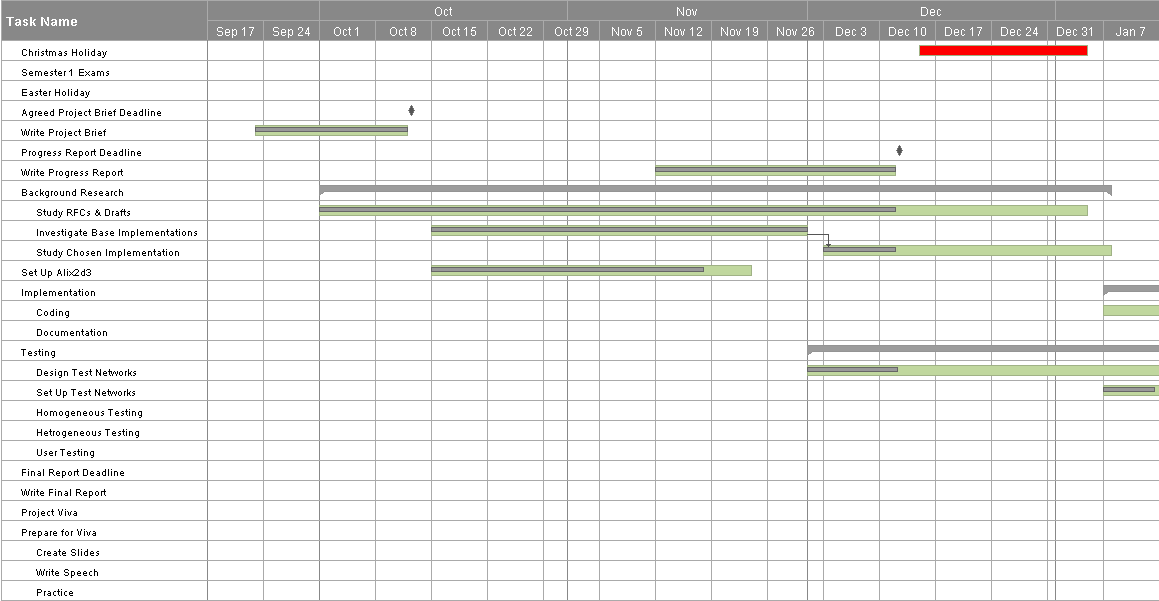
\includegraphics[width=\linewidth]{../Gantt/GanttPart1.png}
\end{center}

\begin{center}
  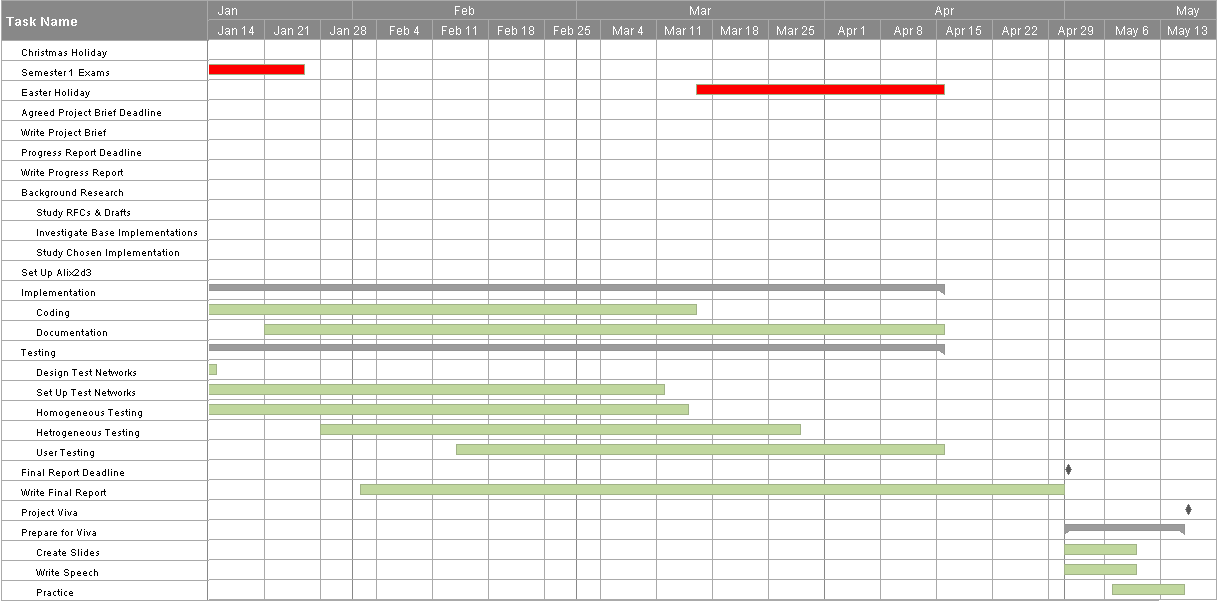
\includegraphics[width=\linewidth]{../Gantt/GanttPart2.png}
\end{center}

\pagebreak

\subsection{Final Gantt Chart}
This Gantt chart shows how I had actually progressed in my project.

\begin{center}
  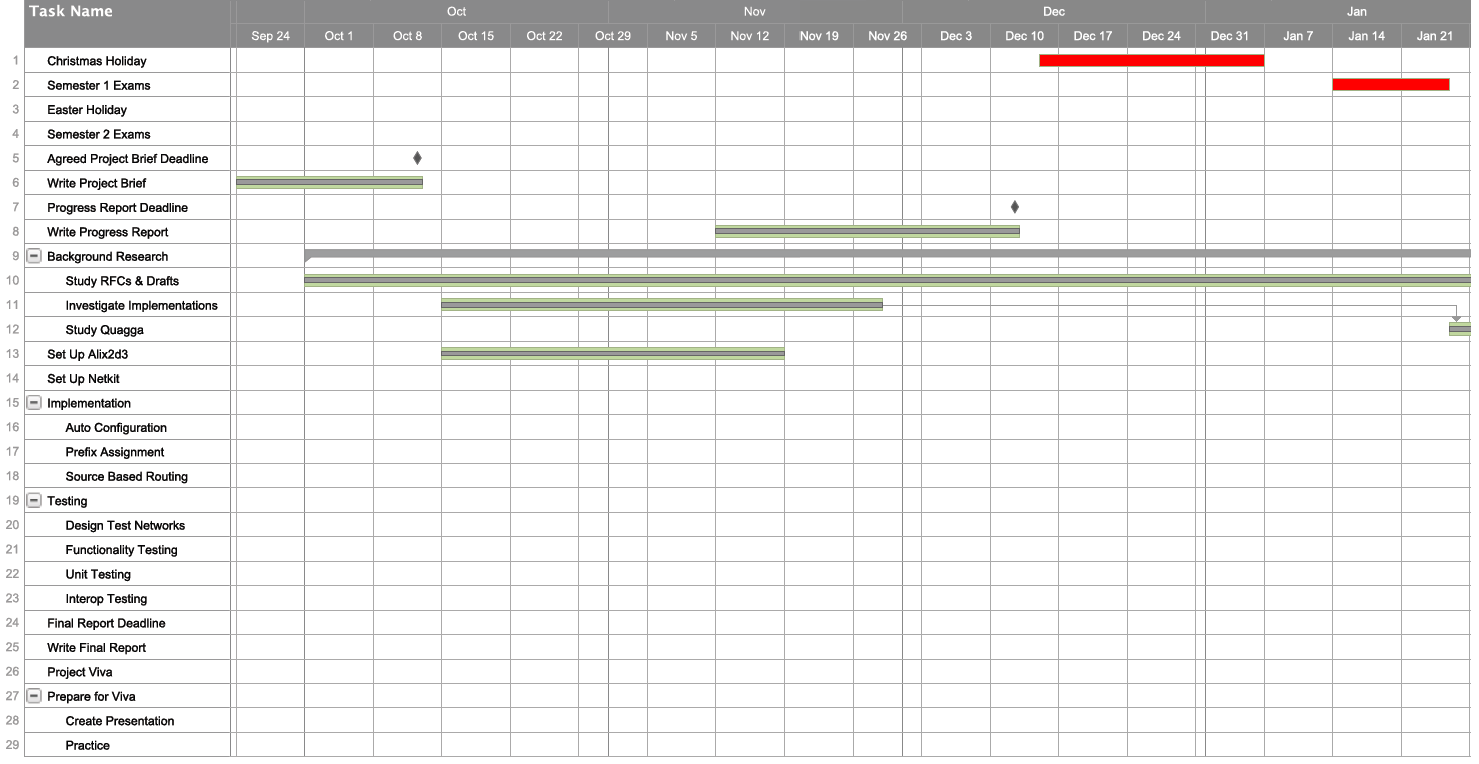
\includegraphics[width=\linewidth]{../Gantt/FinalGanttPt1.png}
\end{center}

\begin{center}
  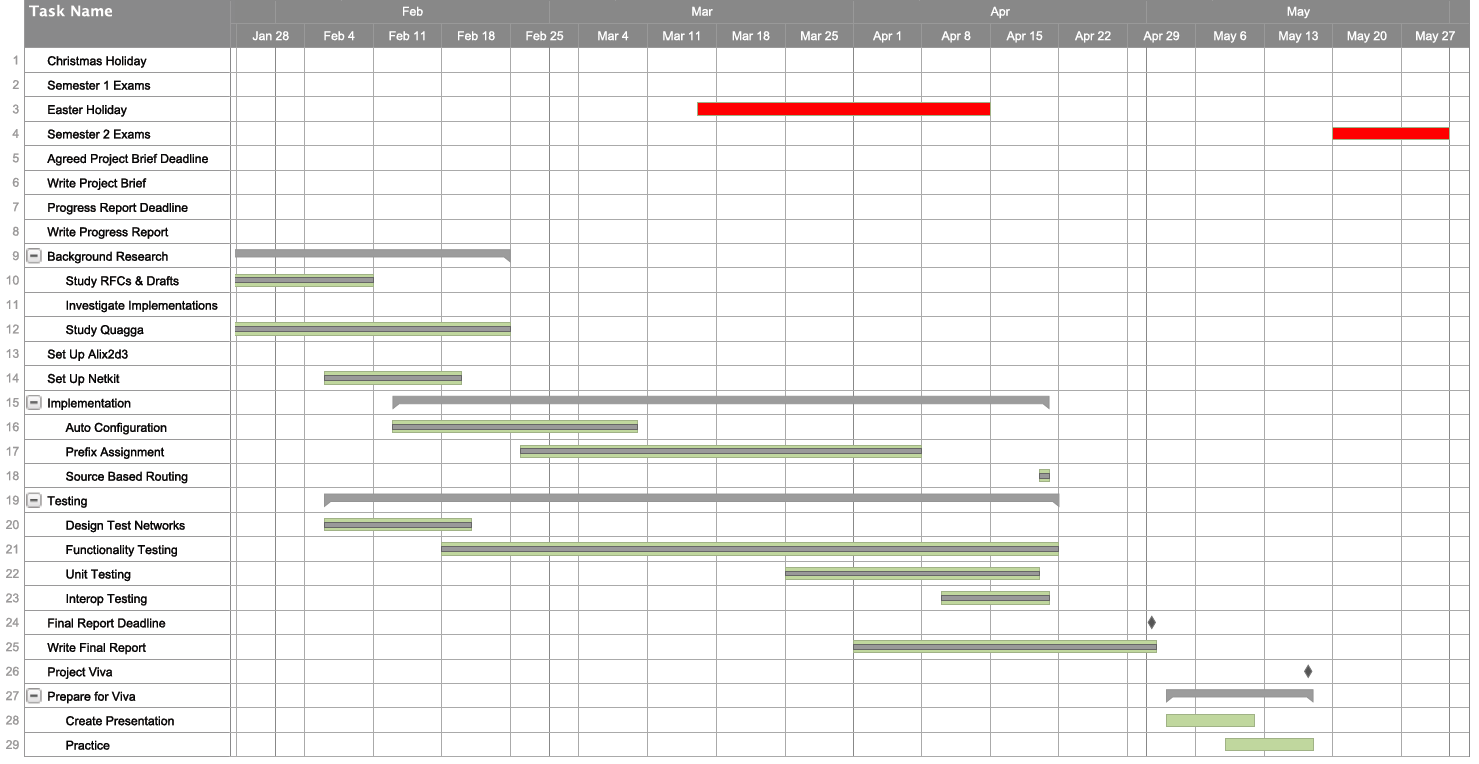
\includegraphics[width=\linewidth]{../Gantt/FinalGanttPt2.png}
\end{center}

\end{landscape}

\pagebreak

\subsection{Explanation of Gantt Charts}
The two Gantt charts I have produced have a few diferences. 


\chapter{Evaluation}
\todo{A critical evaluation}

\section{What Went Well?}
In general I felt that project was successful. Although it was difficult, I
managed to complete my implementation only very slightly behind schedule. I
feel that the software I have developed is functional, robust and maintainable.
Hopefully after code review it will be accepted as part of Quagga.

The program that I have produced meets the goals that I originally set; 

I like that I got an opportunity to work in a language, and therefore style of
programming, that I had had little experience using before this project.  I
feel that because of this I have learnt a lot about how to develop programs in
a procedural style rather than an object oriented one. My skills in writing C
code have improved hugely thanks to this project. I am much more confident in
my understanding of pointers and \texttt{struct}s, and in turn, the low level
operation of a computer.  

I also feel much more confident now about working on large projects. Prior to
this project I had looked at the code bases of open source projects and felt
intimidated by the size and style of the code base. I remember feeling unsure
about where the code for these applications even started from. Having completed
this project, I have come to realise that the individual blocks and statements
that make up the large projects, are exactly the same as those that I am very
familiar with in my own work - there is not often anything that when taken in
isolation, I am totally unable to understand.

The final aspect that I feel went well in this project is that I discovered a
huge amount of information about the software projects that exist to support
networking. Not only did I learn about the Quagga project, but I also learnt
about many other projects. I read about and used the competing routing daemon
implementations Bird and XORP\@. I read about Cisco's proprietary implementations of
these protocols too. And I also made use of many other pieces of network
software: I made heavy use of \texttt{iproute2}, the package that has
superseded \texttt{ifconfig} as the de facto way to control TCP/IP networking
in Linux; I also experimented with \texttt{radvd} the Router Advertisement
Daemon; and also played with WIDE-DHCPv6. 

\section{What Could Have Gone Better?}
In general the project went well, perfection however is rarely obtainable, and
there were things that if I was to do this project again, I might have done
differently. 

Firstly, I did not properly dig into the project until later than I would have
liked.  This was partially due to having a very high workload from my other
courses at the end of Semester One - given the chance I would go back in time
and choose less coursework intensive optional modules. The other factor was a
lack of confidence about jumping in at the deep end. With the experience of
working on a project like this I now know that one of the best ways of learning
how a piece of software works is just to try to add a feature to it.

I also feel that I could have become more involved in the discussion about the
drafts, again I think I was held back by a lack of experience and confidence,
having never been involved with the Internet Engineering Task Force or any
other international standards body before. 
 
\chapter{Conclusions and Future Work}
\todo{Conclusions and future work}

\section{Conclusions}
\todo{Add the ambiguities I previously came up with}
In this project I have shown that it is possible to extend Quagga to implement
zero configuration OSPFv3. Along the way I learned a lot. I also uncovered a
few areas of the draft that I feel are slightly ambiguous or under
prescriptive. 

\section{Continuing the project}
Now that the project is over, I plan to continue with the work I have been
doing.  My goal is to have the code that I have written merged back into the
Quagga mainline. Before this can happen, the code will need to go through a
cleanup stage and a series of code reviews to ensure that it is of sufficient
quality, and is relevant to fit with the rest of the Quagga project.

I also hope to be able to attend the 87th IETF meeting that will take place
during the summer holidays. I have applied for the ECS Student Development
fund, to help me fund the trip. If I am able to go it will give me the
opportunity to discuss future work, and participate in interoperability tests.

\section{Future Work}
The scope of my project was fairly large. As it is such a current research
area, and the drafts I have implemented are designed to be very extensible,
there is a large amount of work that could be based on what I have produced. 

\subsection{DHCPv6-PD}
Ideally an implementation of OSPFv3 Prefix Assignment should be able to handle
aggregated prefixes DHCPv6-PD\@. I decided fairly early on in the project that
this would be beyond the scope of the project. 

There are two ways that I would suggest implementing this functionality. The
first is to make use of an existing DHCPv6 Client such as WIDE-DHCPv6, and find
a way to hook into the PD message functionality. The other would be to add
functionality to Quagga itself to handle the DHCPv6-PD messages. 

I feel that adding this functionality to Quagga would be the better solution
since it does not couple Quagga to any other projects. It would however be
likely to require a lot more work to achieve.

\subsection{Source Based Routing}
\todo{Draw attention to the fact that I have actually done this}
In the future it may become more common for households to have more than one
broadband connection. Having a cable connection, with a ADSL line for backup is
a scenario that may become common in the home of the future. 

The issue with this type of set up is that to prevent various attacks, in
accordance with BCP 38, ISPs are likely to drop any traffic that has a source
address that does not fall within the prefix that it allocated to that network.
As such, if multiple ISPs are used, the network traffic must be routed to the
correct ISP. 

Source Based routing is a possible solution to this. Source based routing works
by forwarding traffic based on the source address of the packet, as well as its
destination address. 

I implemented a basic proof of concept as an extension to my main code. The
branched version of the code that I produced is not compatible with the vanilla
autoconfiguration implementation. It is based loosely on drafts by Fred Baker,
a former IETF chair. These drafts specify a set of replacement LSAs for some of
the standard OSPFv3 LSA types, these LSAs are based on Type Length Values
(TLVs) similar to those used in the autoconfiguration draft, rather than the
more rigid specification of standard OSPFv3. Due to the complexity of these
drafts, I decided that within the project not to conform strictly to the
draft.

My implementation worked by exploiting the Linux Kernel's ability to have
multiple routing tables. A routing table is created for each source address
range that will be routed. The systems policy table is then used to select
which routing table to use based on the source address.  

Quagga's Zebra daemon by default ships with the ability to manipulate any
routing table. I extended the Zebra protocol's message for adding entires to
the routing table to include the source address, and then chose the routing
table based on a hash of the source address.  Unfortunately Quagga does not
currently offer any functionality for manipulating the Policy table. To
overcome this I made use of \texttt{iproute2}'s \texttt{ip -6 rule} command,
which I called from a bash shell script, invoked using the \texttt{system}
function. 

This proof of concept shows that Quagga can be extended to implement source
based routing. It is however nowhere nearly a complete solution - firstly it
will not be interoperable with any other implementations as it does not conform
to the draft, and secondly the use of the \texttt{system} system call is
neither secure, elegant nor portable. 

\subsection{Multi-hop Service discovery}
Service discovery has become very popular in modern networks. Its major use
cases include finding media streaming severs and printers on a home network. At
present, a device must be connected to the same subnet as a service for it to
be able to discover it as the service discovery messages are not forwarded by
the router. 

It would be possible for Quagga to be extended to flood these service discovery
messages across the whole network, allowing services on one subnet, to be
accessible from another. Major use cases for this include: monitoring home
appliances from within the home workstation network, and displaying images on a
screen from a guest network.

There are currently no drafts suggesting how this would be done, ideally Apple
Inc.\@ would eventually extend their service discovery platform, Bonjour, to
use this kind of technology.

\subsection{Domain Name Services}
\todo{Expand}
Draft mentions DNS by both stateless DHCP and through RAs. The draft recomends
that each router is set up as a DHCP relay.

\subsection{Security Considerations}
Currently the only security that exists in the implementation is IPSec (IP
level security). It might be beneficial to add an extra layer of security to future 
releases.

Built in security was a feature of OSPFv2 but it was removed in OSPFv3 in favour of 
using IPSec. In some circumstances, IPSec is considered difficult to employ. 
RFC6506 reintroduces OSPF level security through the use of an Authentication 
Trailer. 

This RFC could be implemented to add Security to Autoconfigured networks. It would 
be possible to provide CPE that comes with a randomly generated key similar to the 
randomly generated Wireless PSKs that currently come with wireless access points.

\section{Deployment in the Home}
As IPv6 becomes more common place, and IPv4 is slowly phased out, this project can 
actually be used in the home. For home users to actively switch to IPv6 there needs 
to be some features that they cannot get from IPv4 - I think that this project 
implements one of those features.

Unfortunately though it does not stop at home users, ISPs also need to be on
board.  Currently in the UK there is only a very small number of ISPs who
provide IPv6 addresses to their customers. SixXS list just 7 UK ISPs, the only
one on the list I have heard is Andrews \& Arnold.

Of course these problems are outside of my control, hopefully with time, the
large ISPs will be able to overcome the inertia of switching to IPv6.
 
\pagebreak

\printnomenclature

\addcontentsline{toc}{chapter}{Nomenclature}
\pagebreak

\cleardoublepage
\phantomsection
\addcontentsline{toc}{chapter}{Bibliography}
\bibliography{FinalReport}{}
\bibliographystyle{unsrt}

\appendix 
%\appendixpage

\begin{landscape}
\chapter{Typical Home Networks}
\section{Present}
\label{typical_homenet_present}
\begin{center}
	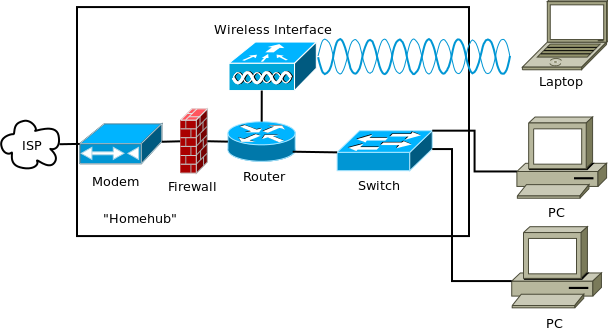
\includegraphics[width=0.75\linewidth]{../Diagrams/Network/TypicalHomenet.png}
\end{center}
This diagram shows a typical home network in the present day. The hardware
inside the box labeled ``Homehub'' is typically provided to customers as one
plug in and play device. It is commonly referred to as a router, although this
is slightly misleading as they perform many other tasks that routing.

As can be seen from the diagram, the box provides the house with wired and
wireless connections to the LAN and the internet. The WLAN is typically bridged
with the LAN to give create a single subnet.

\section{Future}
\label{typical_homenet_future}
\begin{center}
	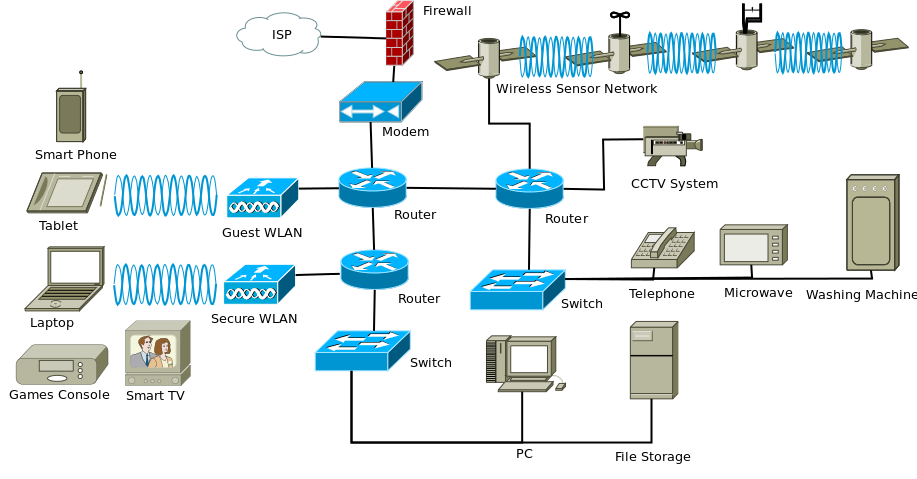
\includegraphics[width=0.9\linewidth]{../Diagrams/Network/FutureHomenet.png}
\end{center}
This diagram shows a hypothetical future home network. The network includes a
guest wireless network, a secured wireless network, a wired network, a network
for appliances, a network for a home surveillance system and a wireless sensor
network.

\chapter{Typical Corporate Network}
\label{typical_corporate_net}
\begin{center}
	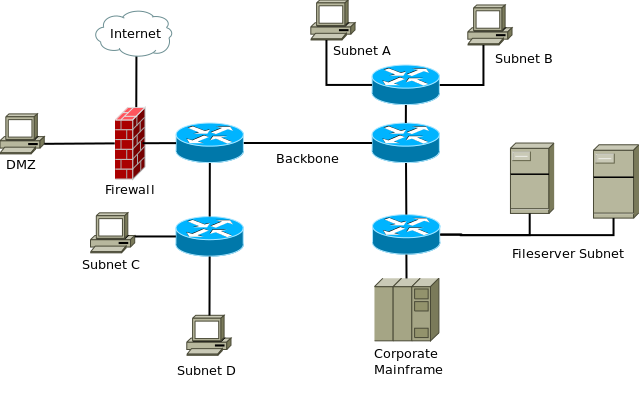
\includegraphics[width=0.75\linewidth]{../Diagrams/Network/CorporateNetwork.png}
\end{center}
This diagram shows the typical topology of a corporate network. For the sake of reducing complexity, Layer 2 switches have not been shown.

\end{landscape}

\chapter{Packets}
Images created with http://interactive.blockdiag.com/packetdiag/

\section{Auto Configuration LSA}
\label{AC-LSA}
\begin{center}
	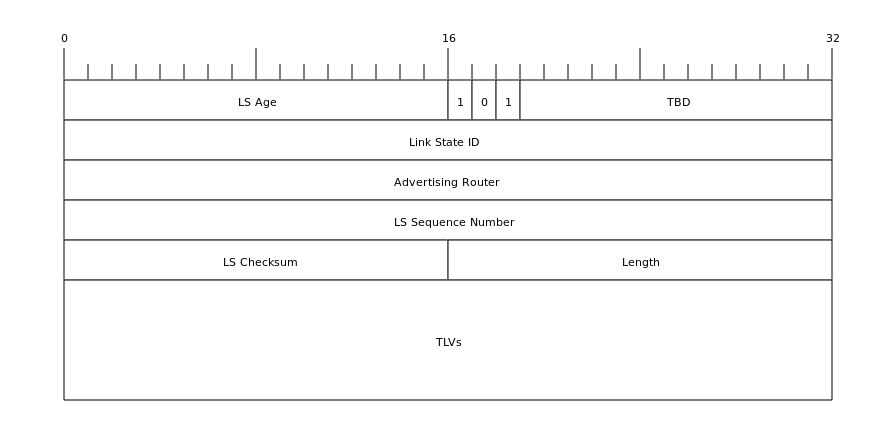
\includegraphics[width=\linewidth]{../Diagrams/Packets/ac_lsa.png}
\end{center}

\section{TLV}
\label{TLV}
\begin{center}
	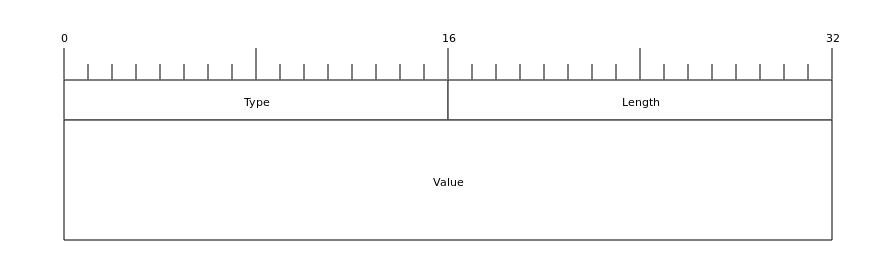
\includegraphics[width=\linewidth]{../Diagrams/Packets/tlv.png}
\end{center}

\section{Router Hardware Fingerprint TLV}
\begin{center}
	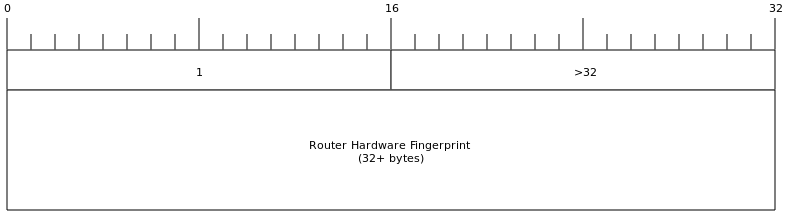
\includegraphics[width=\linewidth]{../Diagrams/Packets/rhwfp_tlv.png}
\end{center}

\section{Aggregated Prefix TLV}
\begin{center}
	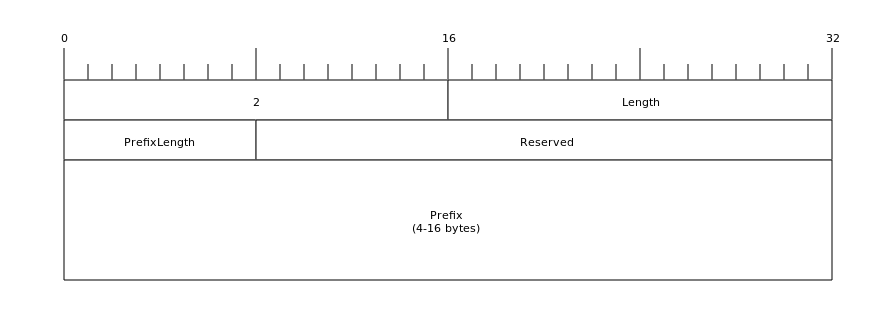
\includegraphics[width=\linewidth]{../Diagrams/Packets/aggregated_prefix_tlv.png}
\end{center}

\section{Assigned Prefix TLV}
\begin{center}
	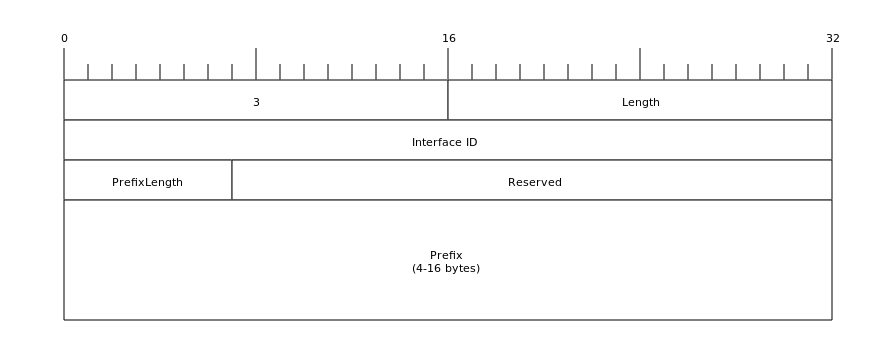
\includegraphics[width=\linewidth]{../Diagrams/Packets/assigned_prefix_tlv.png}
\end{center}

\chapter{Netkit Test Networks}

\section{Simple Network}
\begin{center}
	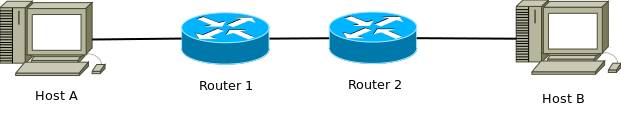
\includegraphics[width=\linewidth]{../Diagrams/Network/SimpleNetkit.png}
\end{center}

\section{Main Network}
\begin{center}
	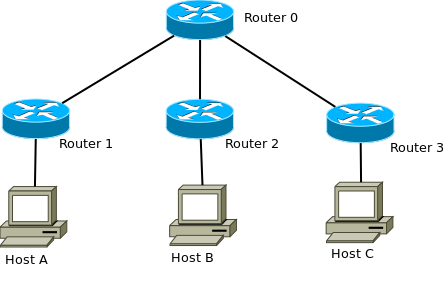
\includegraphics[width=\linewidth]{../Diagrams/Network/MainNetkit.png}
\end{center}

\chapter{Github Stats}
\label{GithubStats}

\section{Github Commit Graph}
\begin{center}
	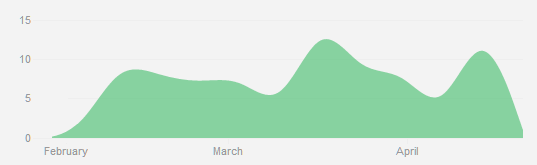
\includegraphics[width=\linewidth]{../Diagrams/Stats/GitHubCommitGraph.png}
\end{center}

\section{Github Punchcard}
\begin{center}
	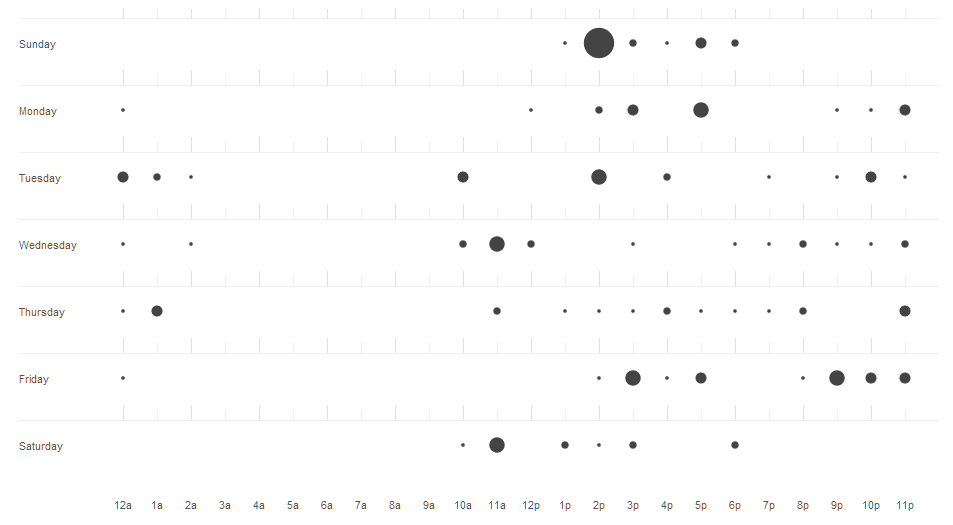
\includegraphics[width=\linewidth]{../Diagrams/Stats/GitHubPunchCard.png}
\end{center}

\chapter{Alix2d3}
As the project progressed it became clear that they Alix2d3s were not as useful
as was originaly believed, thanks to discovery of the briliant software package
Netkit. I did however undertake testing on the Alix2d3s. If someone wished to
repeat my experimentation, the following guides would be helpful. 

\section{Installation Guide}

 This guide\cite{germanGuide} offered a comprehensive list of steps that need to
 be taken to install Ubuntu Linux on a PC Engines alix2d3\cite{alix2d3}.  The article is
 written in German but using Google translate I was able to follow it as it is
 mainly a list of shell commands.

 The process begins with installing the compact flash card as a device on an
 existing Ubuntu desktop PC\@. Next the card is partitioned using \texttt{fdisk},
 the card is then formatted as ext2 (a Linux file system type) using
 \texttt{mk2fs}. The card is then mounted in the file system, using
 \texttt{mount} and a small installation of Linux is copied to the card using
 \texttt{debootstrap} to provide a base system.

 Several settings and devices are linked to the flash cards mount point and
 \texttt{chroot} is used to simulate booting into the new install. The required
 configuration files are edited (e.g.\@ network interface settings) and essential
 software packages (such as \texttt{Vim}, \texttt{SSH}, \texttt{sudo}, and
 \texttt{APT}) are installed. A boot loader such as \texttt{GRUB} is also
 installed and configured.

 Next, the flash card is safely removed, and  inserted into the alix2d3. The
 alix2d3 is then powered on. Using a USB to Null Model cable connecting a PC to
 the alix2d3's serial port, a terminal connection can be established using {\bf
 cu}. I had a few problems using this device (\texttt{ttyUSB0}) but I was able to
 fix this problem using \texttt{chown}. This terminal connection can be used to
 aid the boot process and ensure that there are no Magic ELF errors. Once the
 alix2d3 is up and running it is possible to disconnect the serial cable and
 access it over \texttt{SSH} alone.

 \section{Quagga Installation Guide}

 \subsection{Normal Installation}
This is a procedure that has  turned out to be far more difficult that anticipated.

First of all, need to ensure that all the dependencies are present. The easiest
way I have found to do this is to use:

sudo apt-get build-dep quagga

This should fetch all the packages that quagga depends on. I see no reason to
build these from source, since I shall not be modifying them.

It seems that a package called libtool is also needed to ensure installation works.
Not certain this is needed.

\ libreadline also seems to be an issue (mainly with vtysh):

\texttt{sudo apt-get install lib32readline6}

Next it should be possible to run \texttt{\@./bootstrap}. As far as I know this
produces (among other things) the configure script.

Next run the configure script. This [wiki][wiki] suggests that it is best to
move the folders using:

\texttt{sudo \@./configure --sysconfdir=/usr/local/quagga --localstatedir=/usr/local/quagga}

The configure script will prompt you to create a user called quagga. Do this by:

sudo adduser quagga
sudo mkdir /usr/local/quagga
sudo chown quagga:quagga /usr/local/quagga

It is now time to run make. See the crosscompiling document for more
information about this. Previously I had issues with zebra making, to fix this
manually editing the Makefile in \@./zebra by adding -lcap to LIBS\@. This doesn't
seem to be a problem with the latest source.

Run sudo make install. This should install everything, and the daemons
should have installed themselves to /usr/local/sbin.

Now a little bit of configuration is required. \texttt{cd /usr/local/quagga}.
Either make a real config file for the daemon, or just create a file containing ``password test''.


You should now be able to run sudo ospf6d. If you can't, try ldconfig.


[wiki]: http://wiki.nil.com/Installing\_and\_running\_Quagga

\subsection{Cross Compilation}

Since Alix2d3s are very slow, a build of Quagga can be incredibly slow. The make parts
alone can take around 15 minutes. (I actually found that XORP had an even slower
compile time, in the order of hours) 

To over come this issue it is possible to compile the source code on a much
faster machine (e.g.\@ desktop pc) and copy it across. 

Since modern machines use a 64bit architecture rather than 32bit like the
Alix2d3s, the compiler must be set up correctly. Adding the cflag ``-m32'' should
suffice, however to be on the safe side, ``-m32 -march=i386'' can be used. 

This should be done by appending '--with-clfags=``-m32 -march=i386i''' to \@./configure.

I initially had problems with this compilation. I resolved the issues by going
back to basics and trying to compile a simple helloworld program for the Alix.
Turns out I was missing ``gcc-multilib''. This can be installed with apt.

\chapter{vtysh}
\label{vtysh}

Commands are added using DEFUN and install.

I added the commands:
\begin{itemize}
  \item show ipv6 ospf6 prefix aggregated
  \item show ipv6 ospf6 prefix allocated 
  \item show ipv6 ospf6 prefix assigned X

  \item enable $>$ configure terminal $>$ ipv6 allocate-prefix X:X::X:X/M
  \item enable $>$ configure terminal $>$ no ipv6 allocate-prefix X:X::X:X/M
\end{itemize}


\end{document}
